% GENERATED FILE - do not hand-edit.
% Source of truth: data/calculus-reviewed/c-2.json in the zenith-website repo.
% Regenerate with: python3 scripts/build_calculus_tex.py
\documentclass[11pt]{article}
\usepackage[utf8]{inputenc}
\usepackage[T1]{fontenc}
\usepackage{amsmath,amssymb}
\usepackage{graphicx}
\usepackage[margin=1in]{geometry}
\graphicspath{{../..//}}
\setlength{\parindent}{0pt}
\setlength{\parskip}{0.6em}
\begin{document}
\section*{Chapter 2: Limits and Continuity --- Practice Exercises C2}

\bigskip\noindent\textbf{A1.}\ Evaluate $\displaystyle\lim_{x\to 2}\dfrac{x^2-4}{x^2+4}$.
\begin{list}{}{\setlength{\leftmargin}{3em}\setlength{\labelwidth}{2.5em}\setlength{\itemsep}{0pt}\setlength{\topsep}{2pt}}
\item[(A)] $1$
\item[(B)] $0$
\item[(C)] $-1/2$
\item[(D)] $\infty$
\end{list}

\bigskip\noindent\textbf{A2.}\ Evaluate $\displaystyle\lim_{x\to \infty}\dfrac{4-x^2}{x^2-1}$.
\begin{list}{}{\setlength{\leftmargin}{3em}\setlength{\labelwidth}{2.5em}\setlength{\itemsep}{0pt}\setlength{\topsep}{2pt}}
\item[(A)] $1$
\item[(B)] $0$
\item[(C)] $-1$
\item[(D)] $\infty$
\end{list}

\bigskip\noindent\textbf{A3.}\ Evaluate $\displaystyle\lim_{x\to 3}\dfrac{x-3}{x^2-2x-3}$.
\begin{list}{}{\setlength{\leftmargin}{3em}\setlength{\labelwidth}{2.5em}\setlength{\itemsep}{0pt}\setlength{\topsep}{2pt}}
\item[(A)] $0$
\item[(B)] $1$
\item[(C)] $1/4$
\item[(D)] $\infty$
\end{list}

\bigskip\noindent\textbf{A4.}\ Evaluate $\displaystyle\lim_{x\to 0}\dfrac{x}{x}$.
\begin{list}{}{\setlength{\leftmargin}{3em}\setlength{\labelwidth}{2.5em}\setlength{\itemsep}{0pt}\setlength{\topsep}{2pt}}
\item[(A)] $1$
\item[(B)] $0$
\item[(C)] $-1$
\item[(D)] nonexistent
\end{list}

\bigskip\noindent\textbf{A5.}\ Evaluate $\displaystyle\lim_{x\to 2}\dfrac{x^3-8}{x^2-4}$.
\begin{list}{}{\setlength{\leftmargin}{3em}\setlength{\labelwidth}{2.5em}\setlength{\itemsep}{0pt}\setlength{\topsep}{2pt}}
\item[(A)] $1$
\item[(B)] $3$
\item[(C)] $6$
\item[(D)] $\infty$
\end{list}

\bigskip\noindent\textbf{A6.}\ Evaluate $\displaystyle\lim_{x\to \infty}\dfrac{4-x^2}{4x^2-x-2}$.
\begin{list}{}{\setlength{\leftmargin}{3em}\setlength{\labelwidth}{2.5em}\setlength{\itemsep}{0pt}\setlength{\topsep}{2pt}}
\item[(A)] $-2$
\item[(B)] $-1/4$
\item[(C)] $1$
\item[(D)] $2$
\end{list}

\bigskip\noindent\textbf{A7.}\ Evaluate $\displaystyle\lim_{x\to -\infty}\dfrac{5x^3+27}{20x^2+10x+9}$.
\begin{list}{}{\setlength{\leftmargin}{3em}\setlength{\labelwidth}{2.5em}\setlength{\itemsep}{0pt}\setlength{\topsep}{2pt}}
\item[(A)] $-\infty$
\item[(B)] $-1$
\item[(C)] $3$
\item[(D)] $\infty$
\end{list}

\bigskip\noindent\textbf{A8.}\ Evaluate $\displaystyle\lim_{x\to \infty}\dfrac{3x^2+27}{x^3-27}$.
\begin{list}{}{\setlength{\leftmargin}{3em}\setlength{\labelwidth}{2.5em}\setlength{\itemsep}{0pt}\setlength{\topsep}{2pt}}
\item[(A)] $0$
\item[(B)] $1$
\item[(C)] $3$
\item[(D)] $\infty$
\end{list}

\bigskip\noindent\textbf{A9.}\ Evaluate $\displaystyle\lim_{x\to \infty}\dfrac{2^{-x}}{2^x}$.
\begin{list}{}{\setlength{\leftmargin}{3em}\setlength{\labelwidth}{2.5em}\setlength{\itemsep}{0pt}\setlength{\topsep}{2pt}}
\item[(A)] $-1$
\item[(B)] $1$
\item[(C)] $0$
\item[(D)] $\infty$
\end{list}

\bigskip\noindent\textbf{A10.}\ Evaluate $\displaystyle\lim_{x\to -\infty}\dfrac{2^{-x}}{2^x}$.
\begin{list}{}{\setlength{\leftmargin}{3em}\setlength{\labelwidth}{2.5em}\setlength{\itemsep}{0pt}\setlength{\topsep}{2pt}}
\item[(A)] $-1$
\item[(B)] $1$
\item[(C)] $0$
\item[(D)] $\infty$
\end{list}

\bigskip\noindent\textbf{A11.}\ Evaluate $\displaystyle\lim_{x\to 0}\dfrac{\sin5x}{x}$.
\begin{list}{}{\setlength{\leftmargin}{3em}\setlength{\labelwidth}{2.5em}\setlength{\itemsep}{0pt}\setlength{\topsep}{2pt}}
\item[(A)] $1/5$
\item[(B)] $1$
\item[(C)] $5$
\item[(D)] does not exist
\end{list}

\bigskip\noindent\textbf{A12.}\ Evaluate $\displaystyle\lim_{x\to 0}\dfrac{\sin2x}{3x}$.
\begin{list}{}{\setlength{\leftmargin}{3em}\setlength{\labelwidth}{2.5em}\setlength{\itemsep}{0pt}\setlength{\topsep}{2pt}}
\item[(A)] $2/3$
\item[(B)] $1$
\item[(C)] $3/2$
\item[(D)] does not exist
\end{list}

\bigskip\noindent\textbf{A13.}\ The graph of $y=\arctan x$ has
\begin{list}{}{\setlength{\leftmargin}{3em}\setlength{\labelwidth}{2.5em}\setlength{\itemsep}{0pt}\setlength{\topsep}{2pt}}
\item[(A)] vertical asymptotes at $x=0$ and $x=\pi$
\item[(B)] horizontal asymptotes at $y=\pm\pi/2$
\item[(C)] horizontal asymptotes at $y=0$ and $y=\pi$
\item[(D)] vertical asymptotes at $x=\pm\pi/2$
\end{list}

\bigskip\noindent\textbf{A14.}\ The graph of $y=\dfrac{x^2-9}{3x-9}$ has
\begin{list}{}{\setlength{\leftmargin}{3em}\setlength{\labelwidth}{2.5em}\setlength{\itemsep}{0pt}\setlength{\topsep}{2pt}}
\item[(A)] a vertical asymptote at $x=3$
\item[(B)] a horizontal asymptote at $y=1/3$
\item[(C)] a removable discontinuity at $x=3$
\item[(D)] an infinite discontinuity at $x=3$
\end{list}

\bigskip\noindent\textbf{A15.}\ Evaluate $\displaystyle\lim_{x\to0}\dfrac{\sin x}{x^2+3x}$.
\begin{list}{}{\setlength{\leftmargin}{3em}\setlength{\labelwidth}{2.5em}\setlength{\itemsep}{0pt}\setlength{\topsep}{2pt}}
\item[(A)] $1$
\item[(B)] $1/3$
\item[(C)] $3$
\item[(D)] $\infty$
\end{list}

\bigskip\noindent\textbf{A16.}\ Evaluate $\displaystyle\lim_{x\to0}\sin\dfrac1x$.
\begin{list}{}{\setlength{\leftmargin}{3em}\setlength{\labelwidth}{2.5em}\setlength{\itemsep}{0pt}\setlength{\topsep}{2pt}}
\item[(A)] $\infty$
\item[(B)] $1$
\item[(C)] $-1$
\item[(D)] nonexistent
\end{list}

\bigskip\noindent\textbf{A17.}\ Which statement is true about $y=\dfrac{2x^2+4}{2+7x-4x^2}$?
\begin{list}{}{\setlength{\leftmargin}{3em}\setlength{\labelwidth}{2.5em}\setlength{\itemsep}{0pt}\setlength{\topsep}{2pt}}
\item[(A)] $x=-1/4$ is a vertical asymptote
\item[(B)] $x=1$ is a vertical asymptote
\item[(C)] $y=-1/4$ is a horizontal asymptote
\item[(D)] $y=2$ is a horizontal asymptote
\end{list}

\bigskip\noindent\textbf{A18.}\ Evaluate $\displaystyle\lim_{x\to\infty}\dfrac{2x^2+1}{(2-x)(2+x)}$.
\begin{list}{}{\setlength{\leftmargin}{3em}\setlength{\labelwidth}{2.5em}\setlength{\itemsep}{0pt}\setlength{\topsep}{2pt}}
\item[(A)] $-2$
\item[(B)] $1$
\item[(C)] $2$
\item[(D)] nonexistent
\end{list}

\bigskip\noindent\textbf{A19.}\ Evaluate $\displaystyle\lim_{x\to0}\dfrac{|x|}{x}$.
\begin{list}{}{\setlength{\leftmargin}{3em}\setlength{\labelwidth}{2.5em}\setlength{\itemsep}{0pt}\setlength{\topsep}{2pt}}
\item[(A)] $0$
\item[(B)] $1$
\item[(C)] $-1$
\item[(D)] nonexistent
\end{list}

\bigskip\noindent\textbf{A20.}\ Evaluate $\displaystyle\lim_{x\to\infty}x\sin\dfrac1x$.
\begin{list}{}{\setlength{\leftmargin}{3em}\setlength{\labelwidth}{2.5em}\setlength{\itemsep}{0pt}\setlength{\topsep}{2pt}}
\item[(A)] $0$
\item[(B)] $-1$
\item[(C)] $1$
\item[(D)] nonexistent
\end{list}

\bigskip\noindent\textbf{A21.}\ Evaluate $\displaystyle\lim_{x\to\pi}\dfrac{\sin(\pi-x)}{\pi-x}$.
\begin{list}{}{\setlength{\leftmargin}{3em}\setlength{\labelwidth}{2.5em}\setlength{\itemsep}{0pt}\setlength{\topsep}{2pt}}
\item[(A)] $1$
\item[(B)] $0$
\item[(C)] $\pi$
\item[(D)] nonexistent
\end{list}

\bigskip\noindent\textbf{A22.}\ Let $f(x)=\begin{cases}(x^2-1)/(x-1)&x\ne1\\4&x=1\end{cases}$. Which statements are true? I. $\lim_{x\to1}f(x)$ exists. II. $f(1)$ exists. III. $f$ is continuous at $x=1$.
\begin{list}{}{\setlength{\leftmargin}{3em}\setlength{\labelwidth}{2.5em}\setlength{\itemsep}{0pt}\setlength{\topsep}{2pt}}
\item[(A)] I only
\item[(B)] II only
\item[(C)] I and II only
\item[(D)] I, II, and III
\end{list}

\bigskip\noindent\textbf{A23.}\ Let $f(x)=(x^2-x)/(2x)$ for $x\ne0$ and $f(0)=k$. If $f$ is continuous at zero, then $k=$
\begin{list}{}{\setlength{\leftmargin}{3em}\setlength{\labelwidth}{2.5em}\setlength{\itemsep}{0pt}\setlength{\topsep}{2pt}}
\item[(A)] $-1$
\item[(B)] $-1/2$
\item[(C)] $1/2$
\item[(D)] $1$
\end{list}

\bigskip\noindent\textbf{A24.}\ Let $f(x)=3x(x-1)/(x^2-3x+2)$ for $x\ne1,2$, with $f(1)=-3$ and $f(2)=4$. Then $f$ is continuous
\begin{list}{}{\setlength{\leftmargin}{3em}\setlength{\labelwidth}{2.5em}\setlength{\itemsep}{0pt}\setlength{\topsep}{2pt}}
\item[(A)] except at $x=1$
\item[(B)] except at $x=2$
\item[(C)] except at $x=1$ or $2$
\item[(D)] at each real number
\end{list}

\bigskip\noindent\textbf{A25.}\ The graph of $f(x)=4/(x^2-1)$ has
\begin{list}{}{\setlength{\leftmargin}{3em}\setlength{\labelwidth}{2.5em}\setlength{\itemsep}{0pt}\setlength{\topsep}{2pt}}
\item[(A)] one vertical asymptote, at $x=1$
\item[(B)] the $y$-axis as its vertical asymptote
\item[(C)] the $x$-axis as its horizontal asymptote and $x=\pm1$ as vertical asymptotes
\item[(D)] two vertical asymptotes at $x=\pm1$, but no horizontal asymptote
\end{list}

\bigskip\noindent\textbf{A26.}\ The graph of $y=(2x^2+2x+3)/(4x^2-4x)$ has
\begin{list}{}{\setlength{\leftmargin}{3em}\setlength{\labelwidth}{2.5em}\setlength{\itemsep}{0pt}\setlength{\topsep}{2pt}}
\item[(A)] a horizontal asymptote at $y = \dfrac{1}{2}$ but no vertical asymptote
\item[(B)] no horizontal asymptote but two vertical asymptotes, at $x = 0$ and $x = 1$
\item[(C)] a horizontal asymptote at $y = \dfrac{1}{2}$ and two vertical asymptotes, at $x = 0$ and $x = 1$
\item[(D)] a horizontal asymptote at $y = \dfrac{1}{2}$ and two vertical asymptotes, at $x = \pm 1$
\end{list}

\bigskip\noindent\textbf{A27.}\ Let $f(x)=\begin{cases}x^2/x&x\ne0\\0&x=0\end{cases}$. Which statements are true? I. $f(0)$ exists. II. $\lim_{x\to0}f(x)$ exists. III. $f$ is continuous at zero.
\begin{list}{}{\setlength{\leftmargin}{3em}\setlength{\labelwidth}{2.5em}\setlength{\itemsep}{0pt}\setlength{\topsep}{2pt}}
\item[(A)] I only
\item[(B)] II only
\item[(C)] I and II only
\item[(D)] I, II, and III
\end{list}

\bigskip\noindent\textbf{B1.}\ If $[x]=\lfloor x\rfloor$, evaluate $\lim_{x\to1/2}[x]$.
\begin{list}{}{\setlength{\leftmargin}{3em}\setlength{\labelwidth}{2.5em}\setlength{\itemsep}{0pt}\setlength{\topsep}{2pt}}
\item[(A)] $1/2$
\item[(B)] $1$
\item[(C)] $0$
\item[(D)] nonexistent
\end{list}

\bigskip\noindent\textbf{B2.}\ If $[x]=\lfloor x\rfloor$, evaluate $\lim_{x\to-2}[x]$.
\begin{list}{}{\setlength{\leftmargin}{3em}\setlength{\labelwidth}{2.5em}\setlength{\itemsep}{0pt}\setlength{\topsep}{2pt}}
\item[(A)] $-3$
\item[(B)] $-2$
\item[(C)] $-1$
\item[(D)] nonexistent
\end{list}

\bigskip\noindent\textbf{B3.}\ $\displaystyle\lim_{x\to\infty}\sin x$
\begin{list}{}{\setlength{\leftmargin}{3em}\setlength{\labelwidth}{2.5em}\setlength{\itemsep}{0pt}\setlength{\topsep}{2pt}}
\item[(A)] is $-1$
\item[(B)] is infinity
\item[(C)] is zero
\item[(D)] does not exist
\end{list}

\bigskip\noindent\textbf{B4.}\ The function $f(x)=\begin{cases}x^2/x&x\ne0\\0&x=0\end{cases}$
\begin{list}{}{\setlength{\leftmargin}{3em}\setlength{\labelwidth}{2.5em}\setlength{\itemsep}{0pt}\setlength{\topsep}{2pt}}
\item[(A)] is continuous everywhere
\item[(B)] is continuous except at $x = 0$
\item[(C)] has a removable discontinuity at $x = 0$
\item[(D)] has an infinite discontinuity at $x = 0$
\end{list}

\bigskip\noindent\textbf{B5.}\ Let $f(x)=\begin{cases}1-x&-1\le x<0\\2x^2-2&0\le x\le1\\-x+2&1<x<2\\1&x=2\\2x-4&2<x\le3\end{cases}$. $\displaystyle\lim_{x\to2}f(x)$
\begin{list}{}{\setlength{\leftmargin}{3em}\setlength{\labelwidth}{2.5em}\setlength{\itemsep}{0pt}\setlength{\topsep}{2pt}}
\item[(A)] equals $0$
\item[(B)] equals $1$
\item[(C)] equals $2$
\item[(D)] does not exist
\end{list}

\bigskip\noindent\textbf{B6.}\ Let $f(x)=\begin{cases}1-x&-1\le x<0\\2x^2-2&0\le x\le1\\-x+2&1<x<2\\1&x=2\\2x-4&2<x\le3\end{cases}$. The function $f$ is defined on $[-1,3]$
\begin{list}{}{\setlength{\leftmargin}{3em}\setlength{\labelwidth}{2.5em}\setlength{\itemsep}{0pt}\setlength{\topsep}{2pt}}
\item[(A)] if $x \neq 0$
\item[(B)] if $x \neq 1$
\item[(C)] if $x \neq 2$
\item[(D)] at each $x$ in $[-1,3]$
\end{list}

\bigskip\noindent\textbf{B7.}\ Let $f(x)=\begin{cases}1-x&-1\le x<0\\2x^2-2&0\le x\le1\\-x+2&1<x<2\\1&x=2\\2x-4&2<x\le3\end{cases}$. The function $f$ has a removable discontinuity at
\begin{list}{}{\setlength{\leftmargin}{3em}\setlength{\labelwidth}{2.5em}\setlength{\itemsep}{0pt}\setlength{\topsep}{2pt}}
\item[(A)] $x = 0$
\item[(B)] $x = 1$
\item[(C)] $x = 2$
\item[(D)] $x = 3$
\end{list}

\bigskip\noindent\textbf{B8.}\ Let $f(x)=\begin{cases}1-x&-1\le x<0\\2x^2-2&0\le x\le1\\-x+2&1<x<2\\1&x=2\\2x-4&2<x\le3\end{cases}$. On which of the following intervals is $f$ continuous?
\begin{list}{}{\setlength{\leftmargin}{3em}\setlength{\labelwidth}{2.5em}\setlength{\itemsep}{0pt}\setlength{\topsep}{2pt}}
\item[(A)] $-1 \leq x \leq 0$
\item[(B)] $0 < x < 1$
\item[(C)] $1 \leq x \leq 2$
\item[(D)] $2 \leq x \leq 3$
\end{list}

\bigskip\noindent\textbf{B9.}\ Let $f(x)=\begin{cases}1-x&-1\le x<0\\2x^2-2&0\le x\le1\\-x+2&1<x<2\\1&x=2\\2x-4&2<x\le3\end{cases}$. The function $f$ has a jump discontinuity at
\begin{list}{}{\setlength{\leftmargin}{3em}\setlength{\labelwidth}{2.5em}\setlength{\itemsep}{0pt}\setlength{\topsep}{2pt}}
\item[(A)] $x = -1$
\item[(B)] $x = 1$
\item[(C)] $x = 2$
\item[(D)] $x = 3$
\end{list}

\bigskip\noindent\textbf{B10.}\ $\displaystyle\lim_{x\to0}\sqrt{3+\arctan(1/x)}$
\begin{list}{}{\setlength{\leftmargin}{3em}\setlength{\labelwidth}{2.5em}\setlength{\itemsep}{0pt}\setlength{\topsep}{2pt}}
\item[(A)] $\sqrt{3-\pi/2}$
\item[(B)] $\sqrt{3+\pi/2}$
\item[(C)] $\infty$
\item[(D)] does not exist
\end{list}

\bigskip\noindent\textbf{B11.}\ Suppose $\lim_{x\to-3^-}f(x)=\lim_{x\to-3^+}f(x)=-1$ and $f(-3)$ is undefined. Which statements are true? I. $\lim_{x\to-3}f(x)=-1$. II. $f$ is continuous everywhere except at $-3$. III. $f$ has a removable discontinuity at $-3$.
\begin{list}{}{\setlength{\leftmargin}{3em}\setlength{\labelwidth}{2.5em}\setlength{\itemsep}{0pt}\setlength{\topsep}{2pt}}
\item[(A)] I only
\item[(B)] III only
\item[(C)] I and III only
\item[(D)] I, II, and III
\end{list}

\bigskip\noindent\textbf{B12.}\ If $y=1/(2+10^{1/x})$, evaluate $\lim_{x\to0}y$.
\begin{list}{}{\setlength{\leftmargin}{3em}\setlength{\labelwidth}{2.5em}\setlength{\itemsep}{0pt}\setlength{\topsep}{2pt}}
\item[(A)] $0$
\item[(B)] $1/12$
\item[(C)] $1/2$
\item[(D)] does not exist
\end{list}

\bigskip\noindent\textbf{B13.}\ Use the graph of $f$ below. For which listed $a$ do $\lim_{x\to a}f(x)$ and $f(a)$ both exist but differ?
\begin{center}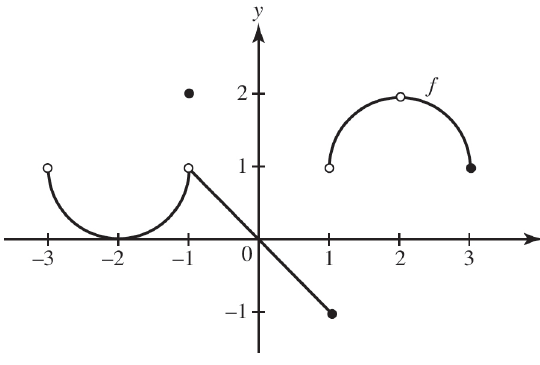
\includegraphics[width=0.6\linewidth]{data/calculus-figures/c2-b13-b15.png}\end{center}
\begin{list}{}{\setlength{\leftmargin}{3em}\setlength{\labelwidth}{2.5em}\setlength{\itemsep}{0pt}\setlength{\topsep}{2pt}}
\item[(A)] $-1$ only
\item[(B)] $2$ only
\item[(C)] $-1$ or $1$ only
\item[(D)] $-1$ or $2$ only
\end{list}

\bigskip\noindent\textbf{B14.}\ Use the graph of $f$ below. For which listed $a$ does $\lim_{x\to a}f(x)$ not exist?
\begin{center}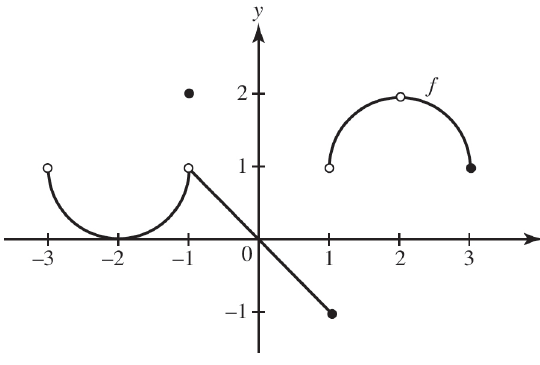
\includegraphics[width=0.6\linewidth]{data/calculus-figures/c2-b13-b15.png}\end{center}
\begin{list}{}{\setlength{\leftmargin}{3em}\setlength{\labelwidth}{2.5em}\setlength{\itemsep}{0pt}\setlength{\topsep}{2pt}}
\item[(A)] $-1$ only
\item[(B)] $1$ only
\item[(C)] $2$ only
\item[(D)] $1$ and $2$ only
\end{list}

\bigskip\noindent\textbf{B15.}\ Use the graph of $f$ below. Which statements are true? I. $\lim_{x\to1^-}f(x)$ exists. II. $\lim_{x\to1^+}f(x)$ exists. III. $\lim_{x\to1}f(x)$ exists.
\begin{center}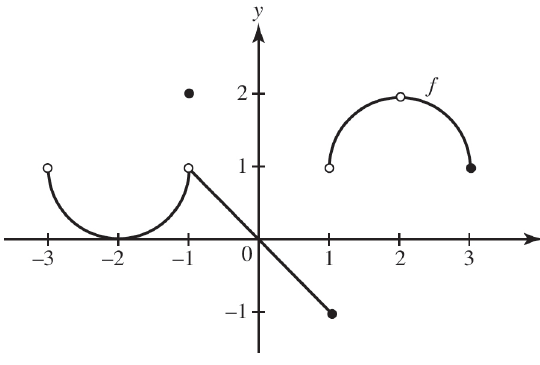
\includegraphics[width=0.6\linewidth]{data/calculus-figures/c2-b13-b15.png}\end{center}
\begin{list}{}{\setlength{\leftmargin}{3em}\setlength{\labelwidth}{2.5em}\setlength{\itemsep}{0pt}\setlength{\topsep}{2pt}}
\item[(A)] I only
\item[(B)] II only
\item[(C)] I and II only
\item[(D)] I, II, and III
\end{list}

\end{document}
